%! TEX root = main.tex

\graphicspath{{00_Images/03_chapter/}}

\chapter{Circuit Analysis: the MXR Distortion+}
\label{ch:mxr}

\section{General Overview and the Cut Technique}
\label{sc:31}

The MXR Distortion+ (model M104, manufactured by MXR/Dunlop) is a commercially produced guitar effects pedal whose signal path is built around a single operational amplifier, the industry-standard \(\mu\)A741, and a pair of diodes that introduce intentional non-linearity.
The pedal accepts a nominal input level of \SI{-22}{\decibel V} (\SI{79}{\milli\volt_{RMS}}) and produces a maximum output level of \SI{-14}{\decibel V} (\SI{200}{\milli\volt_{RMS}}), with a distortion gain range of \SIrange{10}{45}{\decibel} at \SI{1}{\kilo\hertz}.
The complete circuit is shown in figure \ref{fig:mxrOverview}.

\begin{figure}[!htb]
    \centering
    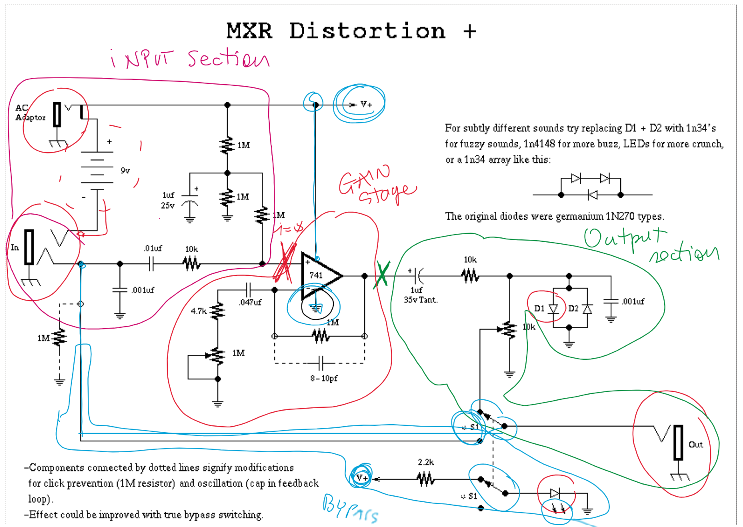
\includegraphics[width=0.90\textwidth]{1.png}
    \caption{Complete schematic of the MXR Distortion+ (M104) with functional regions annotated. The signal path runs from the input jack (left) through the AC coupling network (input section, pink), the 741 gain stage (gain stage, red), the clipping diodes \(D_1\) and \(D_2\) (output section, teal), and finally to the bypass switch \(S_1\) and the output jack. Dotted-line components are modifications for click prevention and oscillation suppression}
    \label{fig:mxrOverview}
\end{figure}

The key circuit features are: the input jack tip is wired to the negative battery terminal so that the battery is disconnected when no cable is inserted, eliminating standby current drain; coupling capacitors block the DC operating point from reaching the source and the load; the AC adaptor jack is wired so that the battery positive terminal floats when the adaptor is connected, preventing two power sources from conflicting; the output impedance of both the Op-Amp stage and the final circuit are intentionally low; and the bypass switch \(S_1\), when closed, routes the dry signal directly to the output while simultaneously illuminating an LED.

\subsection{Decomposing a Complex Circuit: the Cut Technique}

A complex analog circuit like the MXR Distortion+ is not analyzed as a monolithic network.
Instead, it is partitioned into a cascade of simpler subcircuits, each of which can be treated as an LTI block with a well-defined input-output relationship.
The cascade property of LTI systems then allows the overall transfer function to be assembled as the product of the individual transfer functions.
The partitioning relies on identifying suitable cut nodes between stages.
Two types of cut are valid:

\paragraph{High-impedance cut (current cut, \(i \approx 0\))} A cut is placed at a node from which negligible current flows into the following stage.
Because no current is drawn, the voltage at the cut node is unaffected by what follows it, and the two halves of the circuit can be analyzed independently.
Typical locations are the input of a device with very high input impedance, such as the non-inverting input of an Op-Amp in feedback configuration.

\paragraph{Low-impedance cut (voltage cut, \(V = \mathrm{const}\))} A cut is placed at a node that is driven by an ideal or near-ideal voltage source, such as a supply rail or the output of a well-driven voltage buffer.
Because the source impedance is negligibly small, the voltage at the cut node is independent of the current drawn by the following stage.
Applying these two cut types to the MXR Distortion+, the signal path decomposes into the following functional blocks: the supply bias network, the AC input coupling stage, the non-inverting gain stage (linear), and the clipping network (non-linear), as shown in figure \ref{fig:mxrBlocks}.
Each block is characterized by its own transfer function \(TF_1\), \(TF_2\), and \(TF_3\), and the sections that follow treat each in turn.
The block diagram also illustrates the DC level propagating through the chain: a naive calculation using the open-loop input impedance of the 741 predicts a bias of \SI{2.6}{\volt} at the non-inverting input, while the correct closed-loop analysis gives the desired \SI{4.5}{\volt}; this discrepancy is resolved in section \ref{sc:32}.

\begin{figure}[!htb]
    \centering
    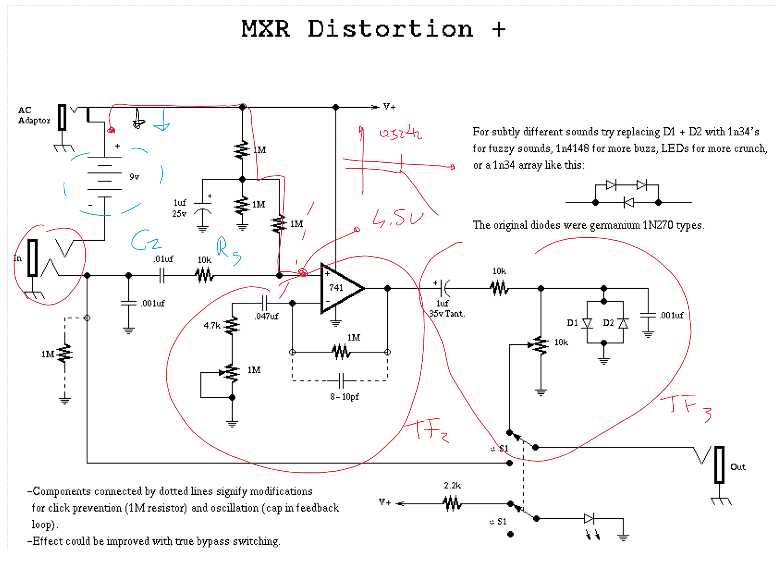
\includegraphics[width=0.90\textwidth]{3.png}
    \caption{Block decomposition of the MXR Distortion+ signal chain. The circuit is partitioned into three functional transfer-function blocks: the input stage (\(TF_1\)), the gain stage (\(TF_2\)), and the output stage (\(TF_3\)). The inset time-domain plots show how the DC level shifts from the raw input, through the \SI{2.6}{\volt} (naive, incorrect) and \SI{4.5}{\volt} (real, closed-loop) bias values, to the final output after AC decoupling}
    \label{fig:mxrBlocks}
\end{figure}

\section{DC Analysis and the Headroom Problem}
\label{sc:32}

In the DC steady state all capacitors are open circuits and all inductors are short circuits.
The signal source itself contributes zero DC voltage when modeled by its Thévenin equivalent, so the DC analysis reduces to finding the quiescent voltages and currents established by the power supply network alone.
Figure \ref{fig:mxrDC} shows the full schematic with all capacitors crossed out (replaced by open circuits) and the DC-relevant quantities annotated.

\begin{figure}[!htb]
    \centering
    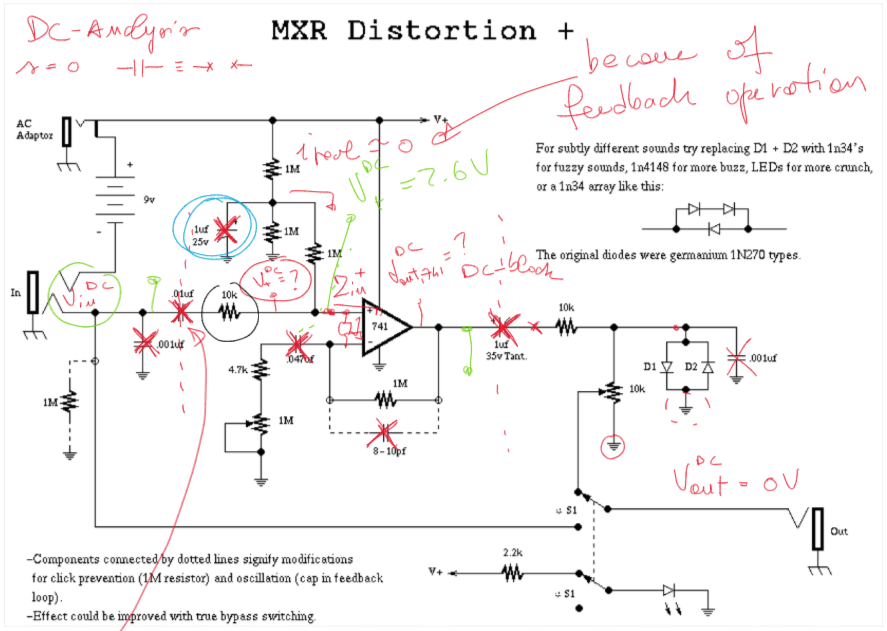
\includegraphics[width=0.90\textwidth]{2.png}
    \caption{DC analysis of the MXR Distortion+ (\(s=0\)). All capacitors are replaced by open circuits (marked with crosses). The notation \(i_{DC}=0\) at the coupling network indicates that the input signal path carries no DC current. The bias node voltage \(V_{DC}=?\) is first naively estimated as \SI{2.6}{\volt} using the datasheet open-loop impedance of the 741; the annotation ``because of feedback operation'' indicates the corrected value of \SI{4.5}{\volt} that results from using the closed-loop impedance. The DC output voltage is \SI{0}{\volt} due to the output AC coupling capacitor}
    \label{fig:mxrDC}
\end{figure}

\subsection{The Need for a Mid-Supply Bias}

The 741 Op-Amp in the MXR Distortion+ is powered from a single \SI{9}{\volt} battery with the negative terminal at ground:
\[
V_{ss}^{-} = \SI{0}{\volt}, \qquad V_{ss}^{+} = \SI{9}{\volt}
\]
The output voltage can swing between the two supply rails, giving a total output dynamic range of \SI{9}{\volt}.
If the quiescent output were at \SI{0}{\volt}, any negative excursion of the audio signal would be immediately clipped against the lower supply rail.
The remedy is to bias the non-inverting input at exactly half the supply voltage:
\[
V_{BIAS} = \frac{V_{ss}^{+}}{2} = \frac{\SI{9}{\volt}}{2} = \SI{4.5}{\volt}
\]
This shifts the entire output waveform upward by \SI{4.5}{\volt}, centring it symmetrically within the available \SI{9}{\volt} window and allowing equal positive and negative excursions of up to \SI{4.5}{\volt} before either supply rail is reached.
The AC output coupling capacitor downstream removes this DC offset before the signal reaches the amplifier or recording device.

\subsection{Calculating the Input Bias Voltage}

The bias voltage is generated by the supply network, which consists of three \SI{1}{\mega\ohm} resistors forming a voltage divider from \(V_{ss}^{+}\) to ground.
The parallel combination of the two lower resistors gives an equivalent lower resistance of \(R_{eq,lower} = \SI{1}{\mega\ohm}  ||  \SI{1}{\mega\ohm} = \SI{0.5}{\mega\ohm}\), so the network presents a Thévenin voltage of:
\[
V_{TH} = V_{ss}^{+} \cdot \frac{R_{eq,lower}}{R_{upper} + R_{eq,lower}} = \SI{9}{\volt} \cdot \frac{0.5}{1 + 0.5} = \SI{3}{\volt}
\]
with a Thévenin resistance of \(R_{TH} = R_{upper}  ||  R_{eq,lower} = \SI{1}{\mega\ohm}  ||  \SI{0.5}{\mega\ohm} = \SI{333}{\kilo\ohm}\).
A first attempt at calculating the voltage at the non-inverting input uses the datasheet value of the 741 open-loop differential input impedance, \(Z_{in}^{OL} \approx \SI{2}{\mega\ohm}\).
Treating this impedance as a shunt load from the \(v^+\) node to ground, the bias voltage would be:
\[
V_{BIAS}^{(naive)} = V_{TH} \cdot \frac{Z_{in}^{OL}}{R_{TH} + Z_{in}^{OL}} = \SI{3}{\volt} \cdot \frac{2}{0.333 + 2} \approx \SI{2.6}{\volt}
\]
This result is significantly below the desired \SI{4.5}{\volt} and would produce heavily asymmetric clipping, as the quiescent output would sit only \SI{2.6}{\volt} above the negative rail and \SI{6.4}{\volt} below the positive rail.
The error in this calculation lies in using the open-loop input impedance.
The 741 is operated in a closed-loop non-inverting configuration with negative feedback.
As established in the theory of negative feedback, the effective input impedance of the non-inverting pin is boosted by the loop gain factor \((1 + A_0 F)\), driving it toward infinity:
\[
Z_{in}^{CL} = Z_{in}^{OL} \cdot (1 + A_0 F) \to \infty
\]
For practical purposes \(Z_{in}^{CL} \to \infty\), which means that the non-inverting input draws negligible current from the bias network.
With \(Z_{in}^{CL} \to \infty\) the bias network sees no load, and the voltage divider formula applies directly:
\[
V_{BIAS}^{(CL)} = V_{ss}^{+} \cdot \frac{R_{eq,lower}}{R_{upper} + R_{eq,lower}} = \SI{9}{\volt} \cdot \frac{0.5}{1.5} = \SI{4.5}{\volt}
\]
The negative feedback thus solves the headroom problem automatically: the closed-loop input impedance is so large that the bias divider is effectively unloaded, and the quiescent point is set precisely at mid-supply.

\section{AC Analysis (\texorpdfstring{\(s > 0\)}{s>0}): Linear Stages}
\label{sc:33}

Once the DC operating point is established, the AC behavior is analyzed by setting all DC sources to zero (replacing voltage sources with short circuits and current sources with open circuits) and treating capacitors with their frequency-dependent impedances \(Z_C = 1/(sC)\).
The cascade of LTI blocks identified by the cut technique can now be characterized individually by their transfer functions.

\subsection{Supply Network: Low-Pass Noise Filter}

The \SI{1}{\micro\farad} capacitor at the junction of the supply resistor network forms a low-pass filter that attenuates any AC noise or ripple present on the \SI{9}{\volt} supply rail before it reaches the non-inverting input.
The pole frequency of this filter is determined by the capacitor and the Thévenin resistance seen looking back into the supply network, which is simply the parallel combination of the two bias resistors:
\[
f_{p,supply} = \frac{1}{2\pi C_1 (R_1  ||  R_2)} = \frac{1}{2\pi \times \SI{1}{\micro\farad} \times \SI{500}{\kilo\ohm}} \approx \SI{320}{\milli\hertz}
\]
The corresponding Bode magnitude plot is shown in figure \ref{fig:mxrSupplyBode}.
This extremely low pole frequency means that any supply noise above a fraction of a hertz, which includes all audible interference, hum, and switching noise, is strongly attenuated before reaching the Op-Amp non-inverting input.
The DC passband gain of this filter is \SI{-6}{\decibel}, reflecting the \(1/2\) voltage division of the equal resistor network.
The bias point is therefore held at a stable, quiet \SI{4.5}{\volt} DC value regardless of noise on the battery or adaptor supply.

\begin{figure}[!htb]
    \centering
    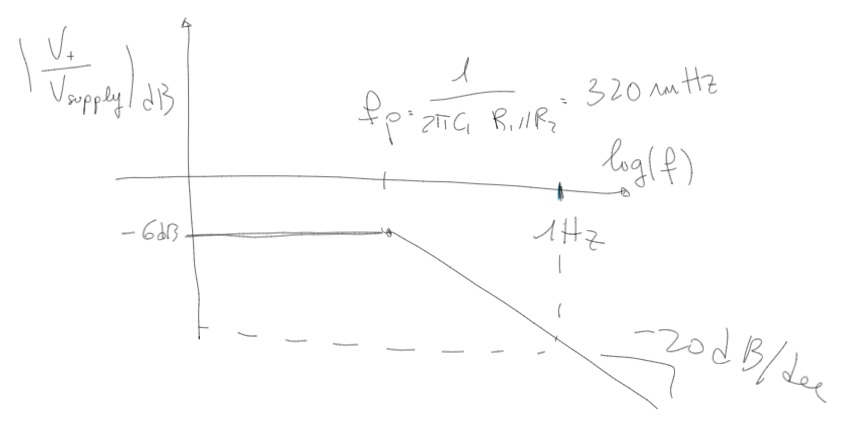
\includegraphics[width=0.90\textwidth]{g4.png}
    \caption{Bode magnitude plot of the supply network low-pass filter. The DC passband gain is \SI{-6}{\decibel} (the equal resistor divider halves the supply voltage). The single pole lies at \(f_p = 1/(2\pi C_1 R_1 || R_2) \approx \SI{320}{\milli\hertz}\), after which the response rolls off at \SI{-20}{\decibel\per decade}, providing strong rejection of all supply noise in the audio band}
    \label{fig:mxrSupplyBode}
\end{figure}

\subsection{Input Stage: AC Coupling Capacitor}

The input coupling capacitor \(C_2 = \SI{0.01}{\micro\farad}\) in series with the \SI{10}{\kilo\ohm} series resistor \(R_S\) forms a high-pass filter that removes any DC component from the guitar signal before it reaches the Op-Amp.
The transfer function has a zero at the origin, associated with the series capacitor blocking DC, and a pole determined by the total resistance in the loop, which is dominated by the high closed-loop input impedance of the bias network:
\[
f_{p,in} = \frac{1}{2\pi C_2 (R_X + R_S)} \approx \SI{1}{\hertz}
\]
where \(R_X \approx \SI{1.5}{\mega\ohm}\) is the effective impedance seen by the capacitor looking toward the bias network.
The corresponding Bode magnitude plot is shown in figure \ref{fig:mxrInputBode}.
The \SI{+20}{\decibel\per decade} rising slope below \SI{1}{\hertz} reflects the zero at the origin, and the response flattens above the pole frequency as the capacitor becomes effectively a short circuit.
The DC gain at high frequency is set by the resistor divider \(R_X/(R_1 + R_X) \approx 1\) since \(R_X \gg R_S\).
This low cutoff ensures that no audible bass content is attenuated: all frequencies of musical interest, from \SI{20}{\hertz} upward, pass through the input stage with negligible attenuation.

\begin{figure}[!htb]
    \centering
    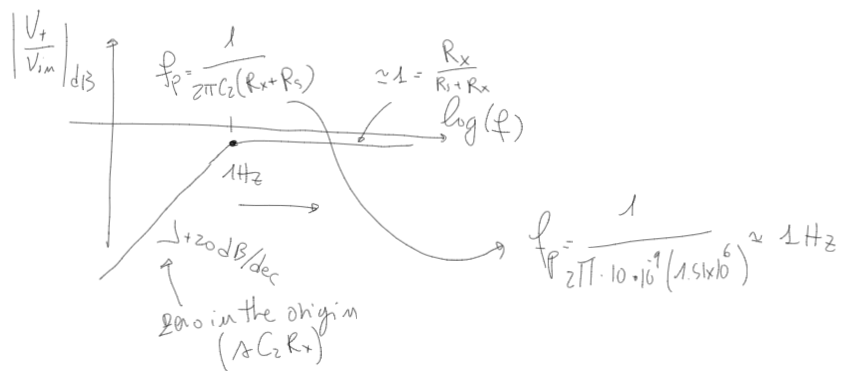
\includegraphics[width=0.90\textwidth]{g5.png}
    \caption{Bode magnitude plot of the input coupling high-pass filter. A zero at the origin produces the \SI{+20}{\decibel\per decade} rising slope at low frequencies, blocking DC from reaching the Op-Amp. The pole at \(f_p = 1/(2\pi C_2(R_X + R_S)) \approx \SI{1}{\hertz}\) marks the transition to the flat passband, ensuring transparent passage of all audio-band content}
    \label{fig:mxrInputBode}
\end{figure}

\subsection{Gain Stage: the Non-Inverting Amplifier and the GBWP Limit}

The 741 is wired in a non-inverting feedback configuration.
The feedback network consists of the \SI{4.7}{\kilo\ohm} resistor \(R_1\) (from the inverting input to ground) and the Distortion potentiometer \(P_1\) (from the Op-Amp output back to the inverting input), which can be set between \SI{0}{\ohm} and approximately \SI{1}{\mega\ohm}.
The closed-loop gain is:
\[
G_{CL} = 1 + \frac{R_{P_1}}{R_1} \qquad \text{with } R_1 = \SI{4.7}{\kilo\ohm}
\]
At minimum potentiometer setting (\(R_{P_1} \to 0\)):
\[
G_{CL}^{min} = 1 \quad (\SI{0}{\decibel})
\]
At maximum potentiometer setting (\(R_{P_1} = \SI{1}{\mega\ohm}\)):
\[
G_{CL}^{max} = 1 + \frac{10^6}{4.7 \times 10^3} \approx 213 \quad (\approx \SI{46.6}{\decibel})
\]
This range matches the datasheet specification of \SIrange{10}{45}{\decibel} distortion gain at \SI{1}{\kilo\hertz}.
An ideal Op-Amp with infinite bandwidth would maintain this flat gain indefinitely at all frequencies, as shown by the ideal Bode curves in figure \ref{fig:mxrGainBode}.
However, the 741 is a compensation-limited amplifier with a Gain-Bandwidth Product of \(\mathrm{GBWP} \approx \SI{1}{\mega\hertz}\).
The closed-loop \SI{-3}{\decibel} bandwidth is:
\[
f_{0,CL} = \frac{\mathrm{GBWP}}{G_{CL}}
\]
At maximum gain the bandwidth collapses to:
\[
f_{0,CL}^{max} = \frac{\SI{1}{\mega\hertz}}{213} \approx \SI{4.7}{\kilo\hertz}
\]
At minimum gain the bandwidth extends to approximately \SI{500}{\kilo\hertz}.
The real Bode curves, accounting for this GBWP limit, are shown alongside the open-loop response \(A(s)\) in figure \ref{fig:mxrGainBode}.
The gain stage therefore acts as an intrinsic low-pass filter whose cutoff frequency is inversely proportional to the gain selected by the user.
At the highest Distortion setting, the amplifier attenuates all frequencies above roughly \SI{4.7}{\kilo\hertz}, which lies within the upper octaves of the guitar frequency range.
This GBWP-limited roll-off is not a design flaw but a tonal characteristic: it contributes to softening the upper harmonics of the distorted waveform, giving the pedal its recognizable warmth at high gain settings.

\begin{figure}[!htb]
    \centering
    \subfloat[Ideal closed-loop gain response]{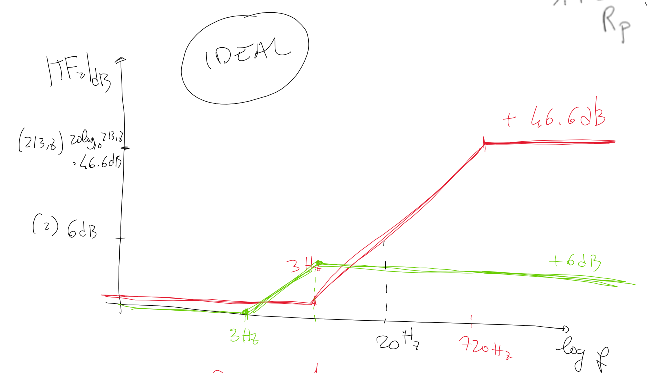
\includegraphics[width=0.47\textwidth]{g6.png}\label{fig:mxrGainIdeal}}
    \hfill
    \subfloat[Real response with GBWP limitation]{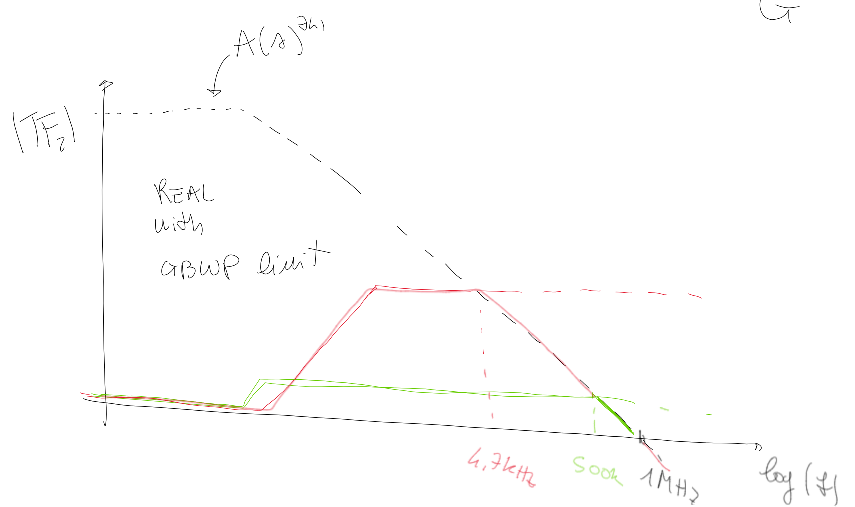
\includegraphics[width=0.47\textwidth]{g7.png}\label{fig:mxrGainReal}}
    \caption{Bode magnitude plots for the non-inverting gain stage. \emph{(a)} Ideal case: the closed-loop gain is flat from DC to infinite frequency at \SI{+46.6}{\decibel} (maximum, red) and \SI{+6}{\decibel} (minimum, green). \emph{(b)} Real case with GBWP \(\approx\) \SI{1}{\mega\hertz}: the open-loop gain \(A(s)\) (dashed) falls at \SI{-20}{\decibel\per decade} from a very low frequency. The closed-loop response tracks the flat plateau only where \(A(s)\) is large enough to sustain the feedback; at maximum gain the \SI{-3}{\decibel} bandwidth collapses to \SI{4.7}{\kilo\hertz}, while at minimum gain it extends to approximately \SI{500}{\kilo\hertz}}
    \label{fig:mxrGainBode}
\end{figure}

\subsection{Output Stage: AC Coupling and Level Control}

After the clipping network, the signal passes through an output AC coupling stage that removes the \SI{4.5}{\volt} DC bias before the signal reaches the output jack.
The output coupling capacitor \(C_5\) in series with the combination of the \SI{10}{\kilo\ohm} series resistor \(R_A\) and the \SI{10}{\kilo\ohm} Level potentiometer \(R_B\) forms a further high-pass filter with pole frequency:
\[
f_{p,out} = \frac{1}{2\pi C_5 (R_A + R_B)} \approx \SI{3}{\hertz}
\]
as illustrated in figure \ref{fig:mxrOutputBode}.
The Level potentiometer \(P_2\) acts as a purely passive voltage divider placed after the diodes.
When \(P_2\) is set to its midpoint, the resistive division produces a flat gain of \(1/2\) (\SI{-6}{\decibel}); when the wiper is at ground, the gain drops to zero (\(-\infty\) \si{\decibel}).
This purely passive attenuation scales the amplitude of the already-distorted signal without affecting the waveform shape or its harmonic content in any way: it changes loudness but not the character of the distortion.

\begin{figure}[!htb]
    \centering
    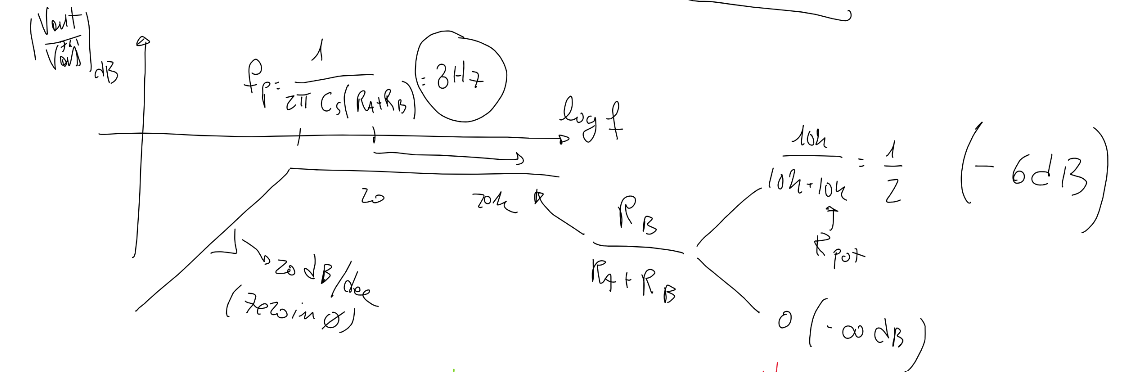
\includegraphics[width=0.90\textwidth]{g8.png}
    \caption{Bode magnitude plot of the output coupling stage. The high-pass pole at \(f_p = 1/(2\pi C_5(R_A + R_B)) \approx \SI{3}{\hertz}\) removes the DC bias from the output. The Level potentiometer \(P_2\) sets the flat-band gain: at mid-travel it produces \SI{-6}{\decibel} (resistive half-division), while at minimum it attenuates the signal to \(-\infty\) \si{\decibel}. The potentiometer is a passive level control that does not alter the distortion character}
    \label{fig:mxrOutputBode}
\end{figure}

\section{Non-Linear Analysis: Diodes and Hard Clipping}
\label{sc:34}

The gain stage alone, without the diodes, produces a clean (linear) amplified signal.
The distinctive character of the MXR Distortion+ arises entirely from the clipping network placed at the output of the Op-Amp, which introduces deliberate, controllable non-linearity into the signal chain.
Non-linear elements such as diodes cannot be analyzed with standard LTI techniques; instead, a piecewise-linear model is adopted that partitions the analysis into separate linear regimes, each valid within a defined range of the signal amplitude.

\subsection{The Diode I-V Characteristic and the Linearised Model}

A real p-n junction diode is governed by the Shockley equation:
\begin{equation}
    I_D = I_S \left(1 - e^{-V_D / V_T}\right)
    \label{eq:shockley}
\end{equation}
where \(I_S\) is the reverse saturation current (of order \SI{}{\nano\ampere} for silicon), \(V_D\) is the voltage across the diode, and \(V_T \approx \SI{25}{\milli\volt}\) is the thermal voltage at room temperature.
The characteristic described by equation~\eqref{eq:shockley} is strongly non-linear: the current is negligibly small for negative or small positive voltages, then rises exponentially once \(V_D\) exceeds a threshold, as shown in figure \ref{fig:diodeIV}.
For circuit analysis purposes, this exponential characteristic is replaced by the piecewise-linear approximation also shown in figure \ref{fig:diodeIV}:

\begin{itemize}
    \item If \(V_D < V_\gamma\): the diode is off and behaves as an open circuit (\(I_D = 0\)).
    \item If \(V_D \geq V_\gamma\): the diode is in full conduction and behaves as an ideal voltage source of \(V_D = V_\gamma\).
\end{itemize}

The threshold \(V_\gamma \approx \SI{0.7}{\volt}\) for silicon diodes; germanium types such as the 1N270 originally fitted in the MXR have a lower threshold of approximately \SI{0.3}{\volt}, which affects the clipping level and thus the tonal character.
This model captures the essential switching behavior of the diode while remaining analytically tractable.

\begin{figure}[!htb]
    \centering
    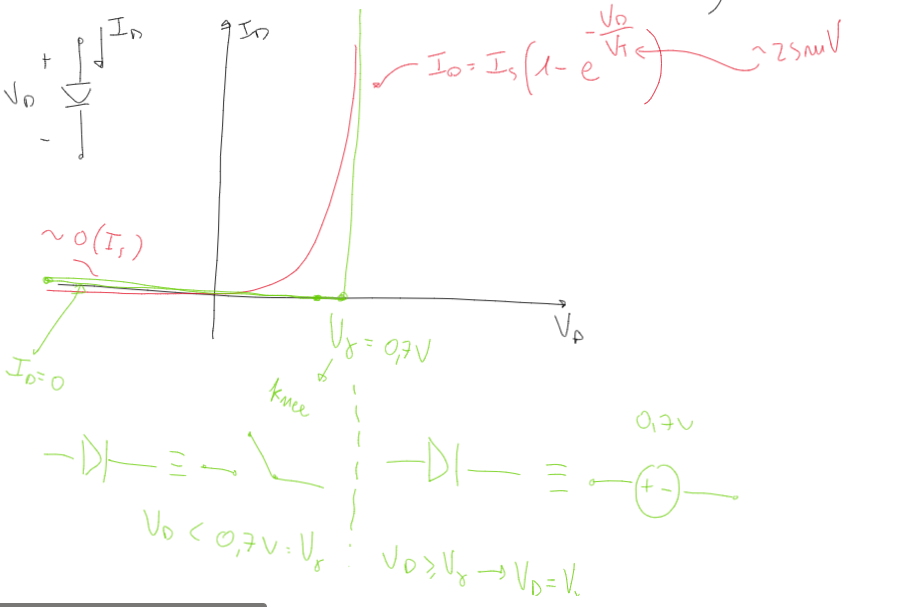
\includegraphics[width=0.90\textwidth]{g9.png}
    \caption{Diode I-V characteristic and piecewise-linear model. The red curve is the Shockley exponential described by equation~\eqref{eq:shockley}; the green lines are the piecewise-linear approximation. For \(V_D < V_\gamma = \SI{0.7}{\volt}\) the diode is modeled as an open circuit (\(I_D = 0\)); for \(V_D \geq V_\gamma\) it is modeled as an ideal \SI{0.7}{\volt} voltage source. The two equivalent circuit symbols corresponding to each region are shown at the bottom of the figure}
    \label{fig:diodeIV}
\end{figure}

\subsection{Clipping Mechanism: Hard Clipping}

In the MXR Distortion+, diodes \(D_1\) and \(D_2\) are connected in anti-parallel between the Op-Amp output node and ground, as illustrated in figure \ref{fig:mxrDiodes}.
Their opposite orientations ensure that each diode is active during a different half-cycle of the signal:

\paragraph{\(D_2\) clips the positive half-cycle} When the AC output voltage rises above \(+V_\gamma = \SI{+0.7}{\volt}\), diode \(D_2\) becomes forward-biased and clamps the output node to \(\SI{+0.7}{\volt}\), shunting the excess current to ground.
All signal content whose instantaneous amplitude exceeds \(+V_\gamma\) is cut off horizontally.

\paragraph{\(D_1\) clips the negative half-cycle} When the AC output voltage falls below \(-V_\gamma = \SI{-0.7}{\volt}\), diode \(D_1\) becomes forward-biased in the reverse direction and clamps the output to \(\SI{-0.7}{\volt}\).
All signal content below this threshold is similarly cut off.
The resulting waveform, shown alongside the unclipped sinusoid in figure \ref{fig:mxrClipping}, has its peaks removed symmetrically, leaving a trapezoidal approximation of the original sinusoid.
The transition from the linear region to the clipped plateau is abrupt, because the diodes switch instantaneously at the threshold; this is the defining characteristic of hard clipping.
In the frequency domain, the sharp corners at the clip points generate a rich spectrum of odd-order harmonics (third, fifth, seventh, and higher) that extend to high orders with significant amplitude, producing the bright, aggressive, sustain-heavy tone characteristic of this pedal.

\begin{figure}[!htb]
    \centering
    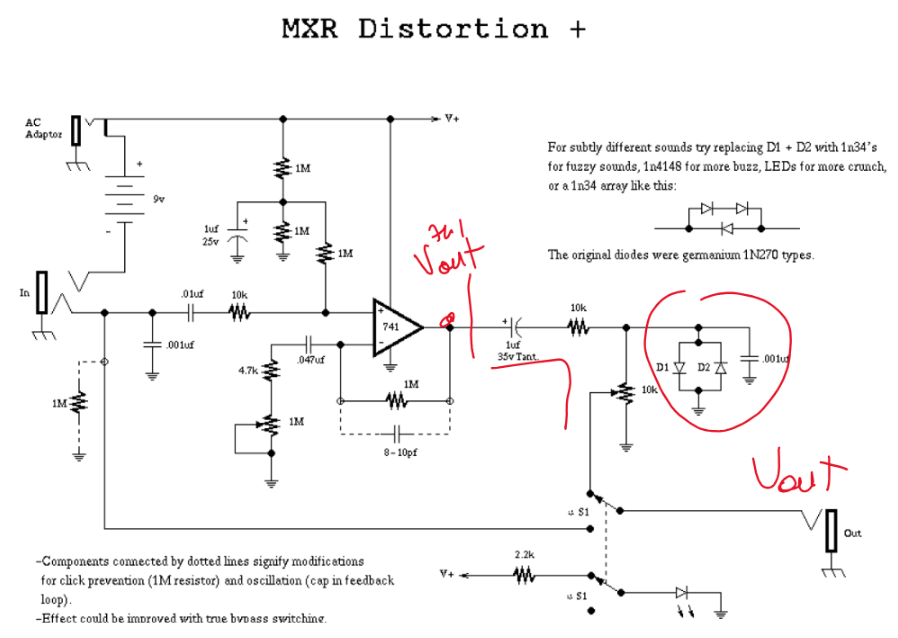
\includegraphics[width=0.90\textwidth]{4.png}
    \caption{Detail of the clipping diode network in the MXR Distortion+. Diodes \(D_1\) and \(D_2\) are connected in anti-parallel between the output node and ground. \(D_2\) clamps positive excursions above \(+V_\gamma\); \(D_1\) clamps negative excursions below \(-V_\gamma\). The \SI{10}{\kilo\ohm} resistor in series limits the current through the clipping node}
    \label{fig:mxrDiodes}
\end{figure}

\begin{figure}[!htb]
    \centering
    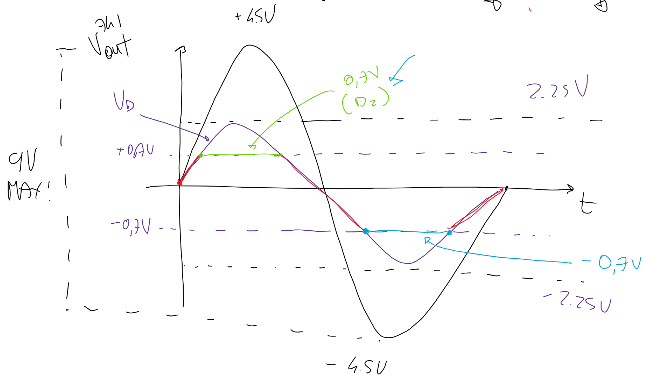
\includegraphics[width=0.90\textwidth]{g10.png}
    \caption{Time-domain waveforms illustrating hard clipping. The black sinusoid represents the Op-Amp output before the diodes, which at maximum gain can reach amplitudes well above \(\pm V_\gamma\) (the figure shows a representative example with peaks at approximately \(\pm \SI{4.5}{\volt}\)). The red/maroon curve is the clipped output, clamped symmetrically at \(+V_\gamma = \SI{+0.7}{\volt}\) by \(D_2\) (upper threshold, green dashed) and at \(-V_\gamma = \SI{-0.7}{\volt}\) by \(D_1\) (lower threshold, blue dashed). The flat-topped waveform approximates a square wave at high gain, producing a harmonic-rich distorted output}
    \label{fig:mxrClipping}
\end{figure}

\subsection{The Role of the Gain and Level Controls}

The Distortion potentiometer \(P_1\) controls how much clipping occurs, and therefore the harmonic content of the output, through a simple but powerful mechanism.
The diode threshold \(V_\gamma = \SI{0.7}{\volt}\) is fixed by the physics of the p-n junction; it is the amplitude of the signal presented to the diodes that the potentiometer controls.
When \(P_1\) is set to a low gain, the signal amplitude at the diode input is small, and only the very peaks of large transients exceed \(V_\gamma\), so little clipping occurs and the output remains nearly clean.
When \(P_1\) is set to a high gain, the signal is amplified to an amplitude far exceeding \(\SI{0.7}{\volt}\); the diodes conduct for a large fraction of each cycle, and the waveform becomes almost completely flat-topped, approximating a square wave and generating a correspondingly rich harmonic spectrum with strong contributions from the third and higher odd harmonics.
In this way the Distortion potentiometer does not simply make the output louder: it controls how deeply the waveform is driven into the non-linear clipping region, setting the ratio between the linear and the clipped portion of each cycle.
The Level potentiometer \(P_2\) acts on a fundamentally different physical principle.
Placed after the diodes and outside the gain loop, it is a purely passive voltage divider that scales the amplitude of the already-distorted signal.
Because the diodes have already shaped the waveform, any rescaling by \(P_2\) affects all harmonic components equally: it changes the overall loudness but leaves the relative harmonic structure, and therefore the timbre and distortion character, completely unaltered.

\subsection{Hard Clipping vs. Soft Clipping}

The MXR Distortion+ implements hard clipping: the diodes are placed outside the feedback loop, connected from the output node directly to ground, so the transition from linear to clipped behavior is instantaneous at the \(V_\gamma\) threshold.
The resulting waveform has sharp corners at the clip points, and the generated harmonics extend to high orders with significant amplitude.
An alternative architecture, exemplified by the Ibanez Tube Screamer, places the clipping diodes inside the Op-Amp feedback loop.
In this configuration the diodes act as a non-linear feedback impedance: as the signal amplitude increases, the effective gain of the stage decreases progressively before the hard clip threshold is reached.
This is called soft clipping.
The waveform corners are rounded rather than sharp, the harmonic spectrum rolls off more rapidly at higher orders, and the overall character is warmer and less aggressive than hard clipping.
Both architectures exploit the non-linearity of the p-n junction; the difference lies in the steepness of the gain compression onset, which determines both the waveform shape at the transition and the high-frequency harmonic content of the distorted signal.